\fancyhead[L]{Chapter III}
\fancyhead[R]{Implementation}

\vspace*{9cm}
\begin{doublespace}
    \centering
    \addcontentsline{toc}{chapter}{Chapter III: Implementation}
    \textbf{ \huge Chapter III \\ [1 cm] Implementation}
\end{doublespace} 

\newpage
\fancyhead[R]{\rightmark}

\setcounter{section}{0}
\section*{Introduction}

This chapter presents the practical implementation of the notification system within the KMS architecture. After establishing the requirements and design in the previous chapters, this phase focused on developing the actual REST API endpoints and WebSocket functionality that enable automated notification management for cryptographic resources. The implementation transforms the theoretical design into a working system, providing the necessary interfaces for users to interact with the notification system.

\section{Tools used}

\subsection{Software Resources:}

\vspace{0.5cm}

\noindent
\begin{minipage}{.7\textwidth}%
    \textbf{IntelliJ IDEA} is an integrated development environment (IDE) developed by JetBrains, mainly used for Java. It offers advanced features such as code auto-completion, project navigation, debugging, refactoring and integration with version control tools, which facilitates the development and maintenance of applications.
\end{minipage}%
\hfill
\begin{minipage}{.20\textwidth}%

\includegraphics[width=.8\textwidth]{images/intellij}
 \end{minipage} \\ \\ \\

\noindent% 
\begin{minipage}{.7\textwidth}%
    \textbf{Bruno} is an API testing and management tool, similar to Postman. It allows sending HTTP requests, analyzing responses and automating tests. Bruno is Git-friendly, and does not save data in the cloud, thus ensuring the confidentiality of information.
\end{minipage}%
\hfill
\begin{minipage}{.22\textwidth}%

\includegraphics[width=\textwidth]{images/bruno.png}
\end{minipage} \\ \\ \\

\noindent
\begin{minipage}{.7\textwidth}%
    \textbf{GitLab} is a web platform for managing Git repositories that allows code versioning, team collaboration and automation of development processes. It offers features such as issue tracking, continuous integration/continuous deployment (CI/CD) and branch management, thus facilitating the development, testing and deployment of software projects.
\end{minipage}%
\hfill
\begin{minipage}{.20\textwidth}%

\includegraphics[width=1\textwidth]{images/gitlab.png}
\end{minipage} \\ \\ \\ 

\noindent% 
\begin{minipage}{.7\textwidth}%
    \textbf{Git} is a version control system used to manage changes made to a computer project. It allows tracking changes, going back if necessary and collaborating effectively with other developers.
\end{minipage}%
\hfill
\begin{minipage}{.20\textwidth}%

\includegraphics[width=\textwidth]{images/git.png}
\end{minipage} \\ \\ \\

\noindent% 
\begin{minipage}{.7\textwidth}%
    \textbf{Rancher Desktop} is an application that allows easy management of container environments on a development workstation. It integrates Kubernetes and containerization tools like containerd or Docker, allowing to create, test and deploy containerized applications locally before sending them to production. Rancher Desktop thus facilitates learning and experimentation with cloud and microservices technologies.
\end{minipage}%
\hfill
\begin{minipage}{.18\textwidth}%

\includegraphics[width=\textwidth]{images/rancher.png}
\end{minipage} \\ \\ \\

\noindent% 
\begin{minipage}{.7\textwidth}%
    \textbf{PostgreSQL} is a powerful and reliable open-source relational database management system. It supports standard SQL and offers advanced features such as transactions, views, stored procedures and extension via custom data types. PostgreSQL is particularly appreciated for its robustness, standards compliance and ability to efficiently handle large amounts of data.
\end{minipage}%
\hfill
\begin{minipage}{.18\textwidth}%

\includegraphics[width=\textwidth]{images/postgresql.png}
\end{minipage} \\ \\ \\

\subsection{Programming languages:}

\vspace{0.5cm}

\noindent% 
\begin{minipage}{.7\textwidth}%
    \textbf{Java} is an object-oriented, versatile and widely used programming language, developed by Sun Microsystems in 1995 (now owned by Oracle). It is designed to be portable, secure and robust, making it a popular choice for developing a variety of applications, from desktop applications to embedded systems through web and mobile applications.
\end{minipage}%
\hfill
\begin{minipage}{.20\textwidth}%

\includegraphics[width=\textwidth]{images/java.png}
\end{minipage} \\ \\ \\ 

\subsection{Frameworks and libraries:}

\vspace{0.5cm}

\noindent% 
\begin{minipage}{.7\textwidth}%
    \textbf{Spring Boot} is a Java framework that simplifies the development of standalone and production-ready applications. It provides automatic configuration, integrated dependencies and tools to quickly create web services, REST APIs and microservices applications, while reducing boilerplate code and facilitating deployment.
\end{minipage}%
\hfill
\begin{minipage}{.20\textwidth}%

\includegraphics[width=\textwidth]{images/spring_boot.png}
\end{minipage} \\ \\ \\

\section{REST API Implementation}

The notification system exposes a comprehensive REST API that enables immediate notification sending, scheduled notification management, and resource status updates. The API follows RESTful principles and integrates seamlessly with the existing KMS architecture.

\subsection{Immediate Notification Endpoint}

The immediate notification endpoint provides the capability to send notifications instantly to users through both email and in-app channels. This endpoint serves as a critical safety mechanism that bypasses the automated Fibonacci scheduling system for emergency situations.

\subsubsection{Purpose and Use Cases}

The immediate notification functionality addresses several critical scenarios that require instant user alerting:

\noindent
\textbf{Emergency Situations:} When cryptographic resources expire unexpectedly soon due to configuration errors or system issues, waiting for the next scheduled processing cycle (every 10 minutes) may be too late. The immediate endpoint ensures that critical alerts reach responsible users within seconds.

\noindent
\textbf{Administrative Interventions:} System administrators can manually trigger notifications for specific resources that may not have been captured by the automated discovery process, or when manual oversight identifies critical situations requiring immediate attention.

\noindent
\textbf{Testing and Validation:} The endpoint serves as a testing mechanism to verify that notification channels are functioning correctly and that users can receive real-time alerts through both email and WebSocket connections.

\subsubsection{Immediate vs Scheduled Notification Flow}

The notification system implements two distinct processing flows:

\noindent
\textbf{Scheduled Flow (Normal Operations):}
Discovery Job → Creates notification records → Processing Job (Fibonacci schedule) → Sends notifications

\noindent
\textbf{Immediate Flow (Emergency/Manual Operations):}
API Call → Instant notification delivery to EMAIL + IN\_APP channels

This dual approach ensures that while the system operates efficiently through automated scheduling for regular expiration management, it maintains the flexibility to handle urgent situations that require immediate user notification.

\subsubsection{Endpoint Specification}

\textbf{POST /v1/notifications/immediate}

This endpoint accepts an immediate notification request and triggers instant delivery through available notification channels. The request requires resource identification, user targeting, and notification content.

\noindent
\textbf{Request Body Structure:}
\begin{itemize}
    \item \textbf{resourceId}: Unique identifier of the cryptographic resource
    \item \textbf{userId}: Target user identifier
    \item \textbf{resourceType}: Type of resource (Certificate or Key)
    \item \textbf{subject}: Notification subject line
    \item \textbf{message}: Detailed notification content
\end{itemize}

\noindent
\textbf{Response:} Returns a list of notification response objects containing the created notification details and delivery status for each enabled channel.

\subsubsection{API Testing with Bruno}

The immediate notification endpoint was thoroughly tested using Bruno to validate request processing and response handling.

\begin{figure}[H]
    \centering
    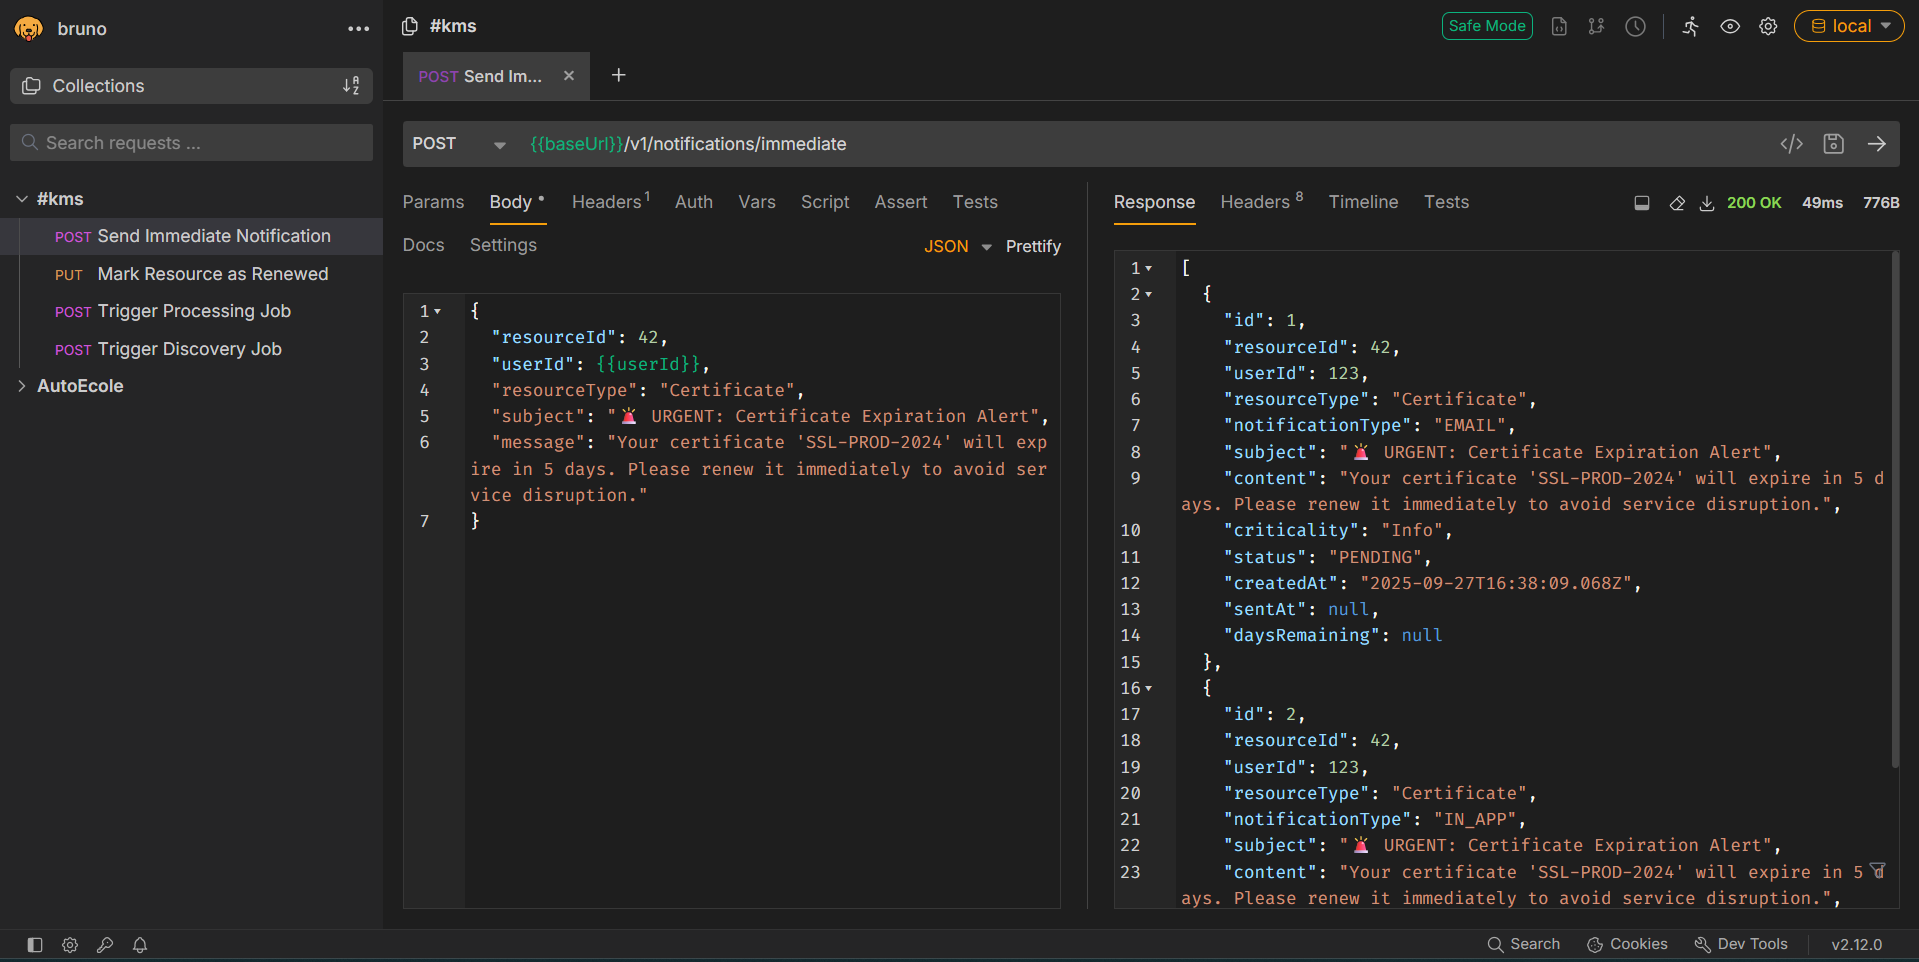
\includegraphics[width=1\textwidth]{images/bruno_immediate_notification.png}
    \caption{Bruno Testing - Immediate Notification Request and Response}
    \label{fig:bruno_immediate}
\end{figure}

The test demonstrates successful processing of an immediate notification request. The response confirms that notifications were created for both email and in-app channels, with unique notification IDs assigned to each channel. The status "PENDING" indicates that the notifications have been queued for processing.

\subsection{Resource Response Endpoint}

This endpoint allows users to mark cryptographic resources as renewed or responded to, which automatically cancels future notifications for those resources.

\subsubsection{Endpoint Specification}

\textbf{PUT /v1/notifications/resource/\{resourceId\}/\{resourceType\}/responded}

This endpoint updates the status of all active notifications for a specific resource, marking them as cancelled when a user indicates they have taken action on the expiring resource.

\noindent
\textbf{Path Parameters:}
\begin{itemize}
    \item \textbf{resourceId}: Unique identifier of the resource
    \item \textbf{resourceType}: Type of the resource (Certificate or Key)
\end{itemize}

\noindent
\textbf{Response:} Returns a confirmation message indicating successful status update.

\subsubsection{Testing Resource Response}

\begin{figure}[H]
    \centering
    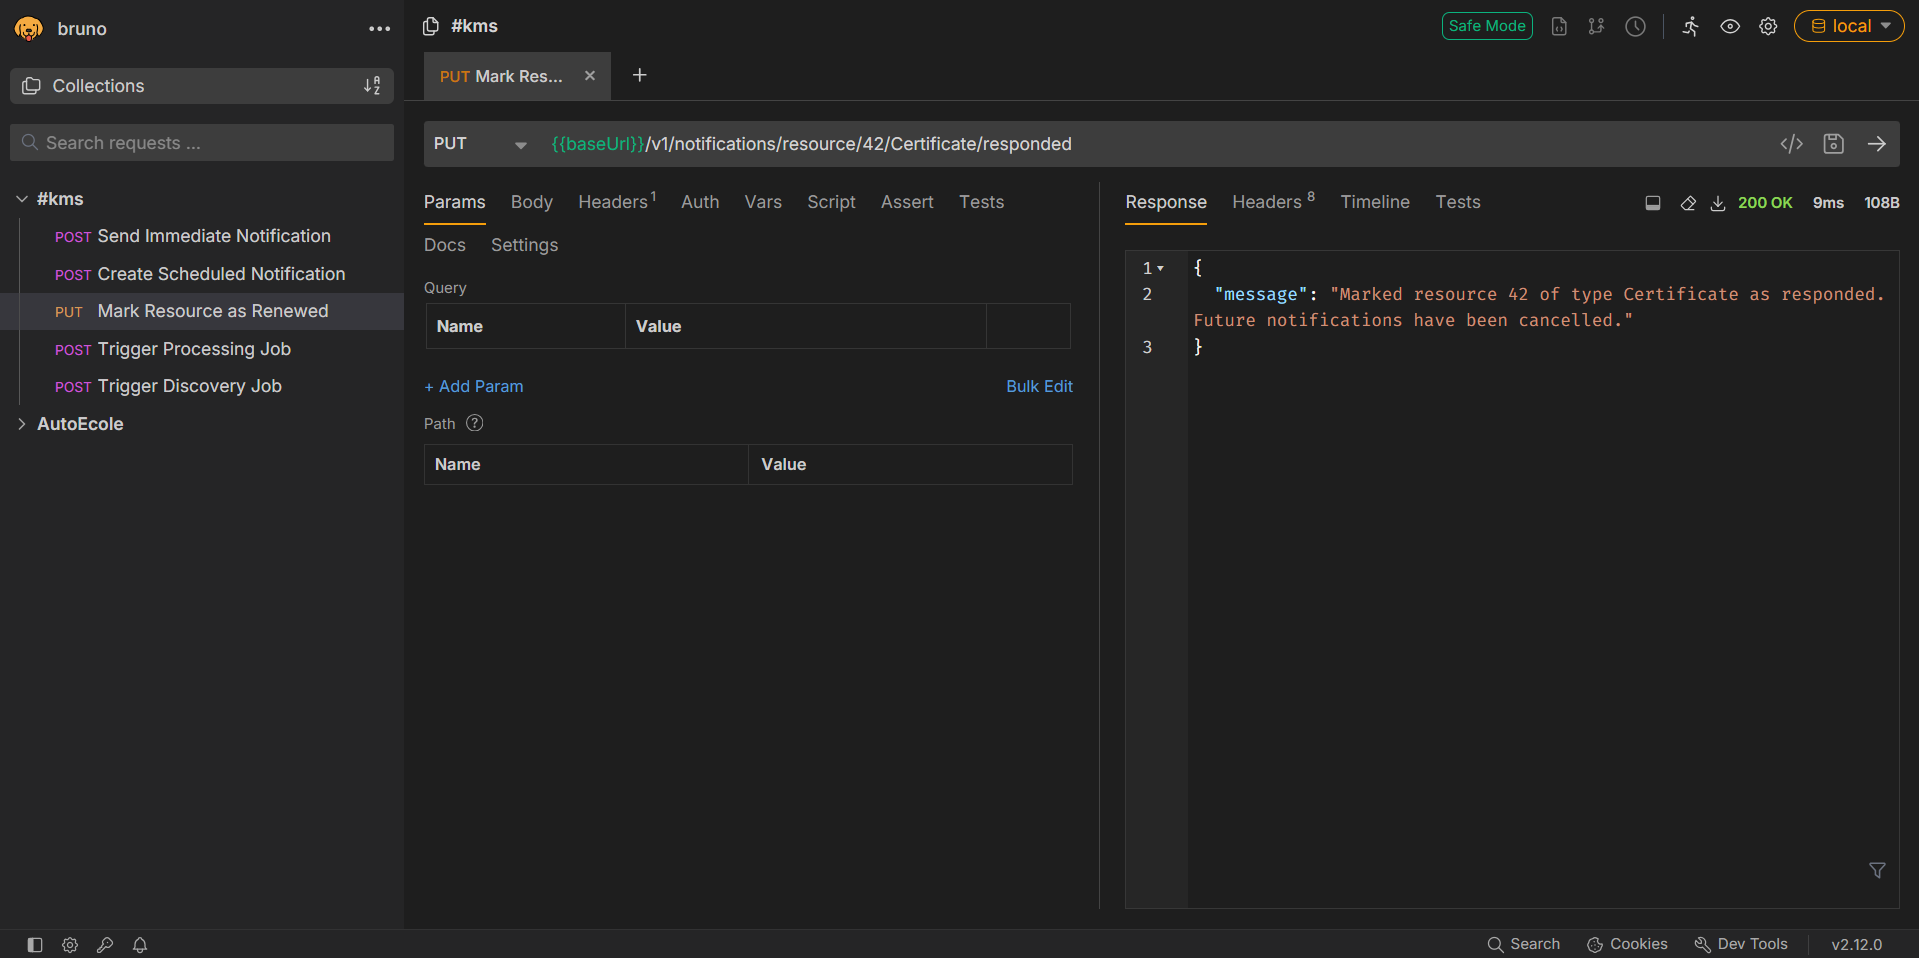
\includegraphics[width=1\textwidth]{images/bruno_resource_response.png}
    \caption{Bruno Testing - Mark Resource as Renewed}
    \label{fig:bruno_resource_response}
\end{figure}

The test confirms that the endpoint successfully processes resource response requests, updating notification statuses and preventing unnecessary future notifications.

\section{WebSocket Implementation}

The WebSocket implementation enables real-time delivery of in-app notifications, providing users with immediate awareness of expiring cryptographic resources.

\subsection{WebSocket Connection Setup}

The WebSocket endpoint is configured to accept connections with user identification, enabling targeted message delivery to specific users.

\subsubsection{Connection Endpoint}

\textbf{WebSocket URL: ws://localhost:8080/ws/notifications?userId=\{userId\}}

The connection requires a userId parameter to identify the target user for notification delivery. Upon successful connection, the system maintains the session and can deliver real-time notifications to the connected user.

\subsection{WebSocket Testing}

Real-time notification delivery was validated using a custom HTML test page that demonstrates WebSocket connectivity and message reception.

\subsubsection{Connection Establishment}

\begin{figure}[H]
    \centering
    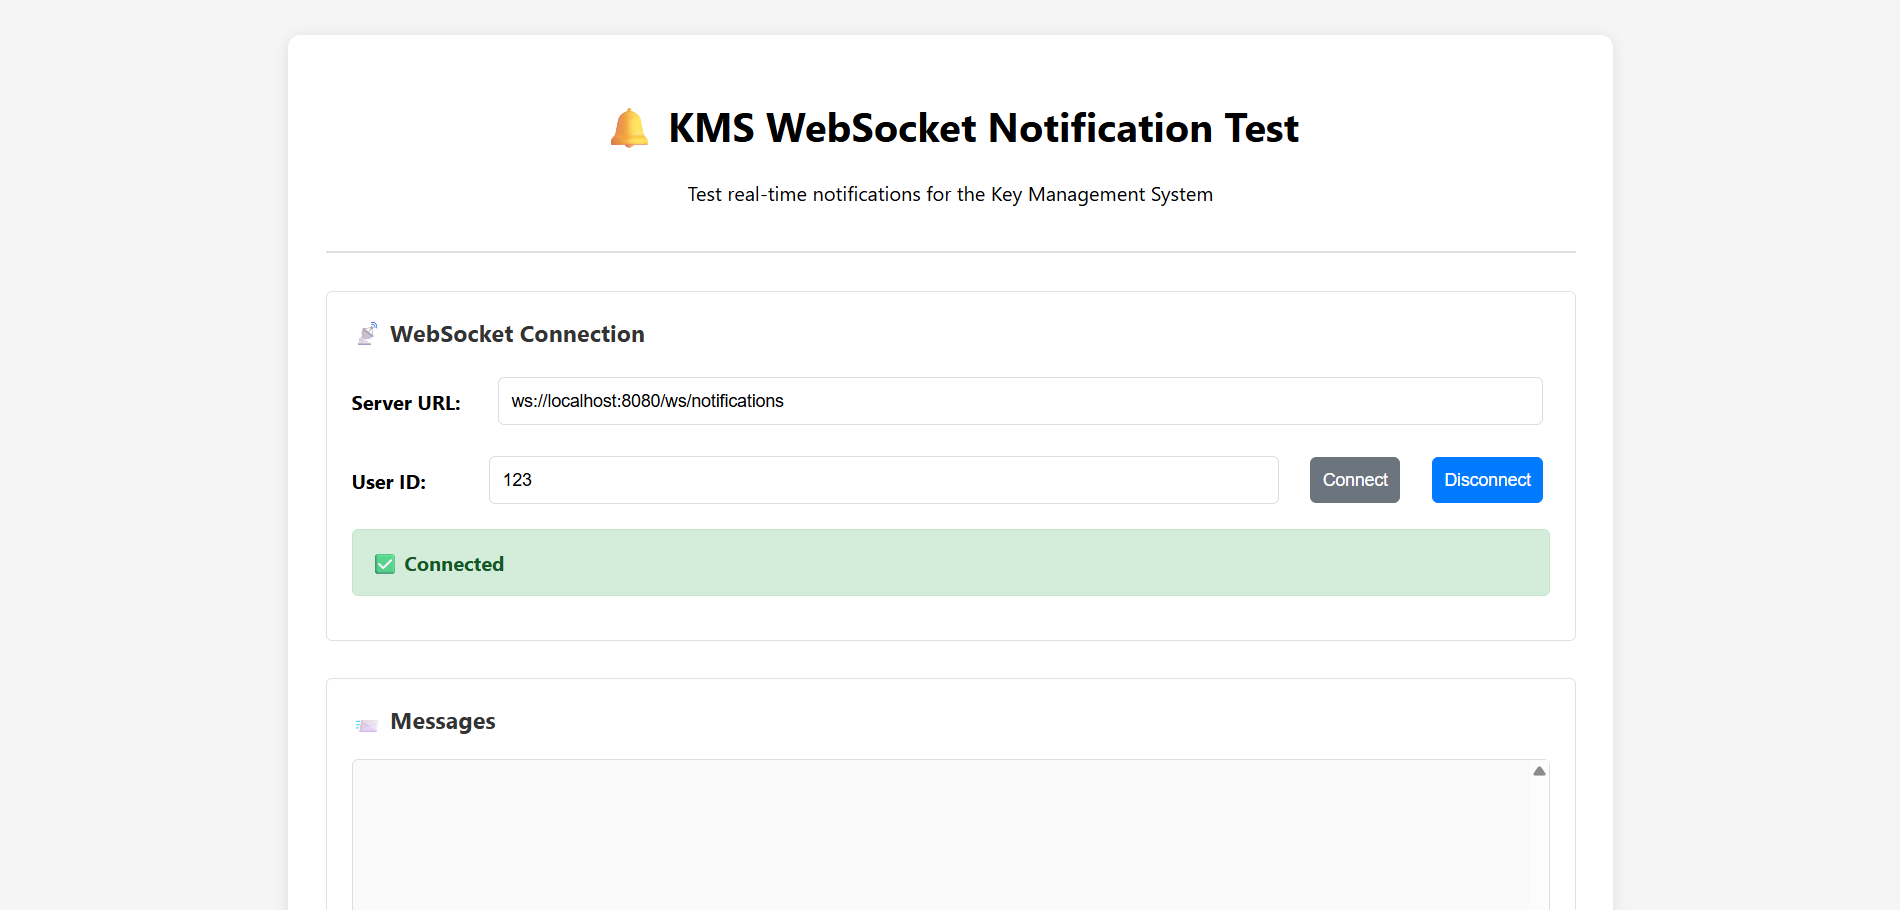
\includegraphics[width=1\textwidth]{images/websocket_connection.png}
    \caption{WebSocket Connection Test Interface}
    \label{fig:websocket_connection}
\end{figure}

The test interface shows successful WebSocket connection establishment with proper user identification. The connection status indicates active communication channel for real-time notification delivery.

\subsubsection{Real-time Message Delivery}

\begin{figure}[H]
    \centering
    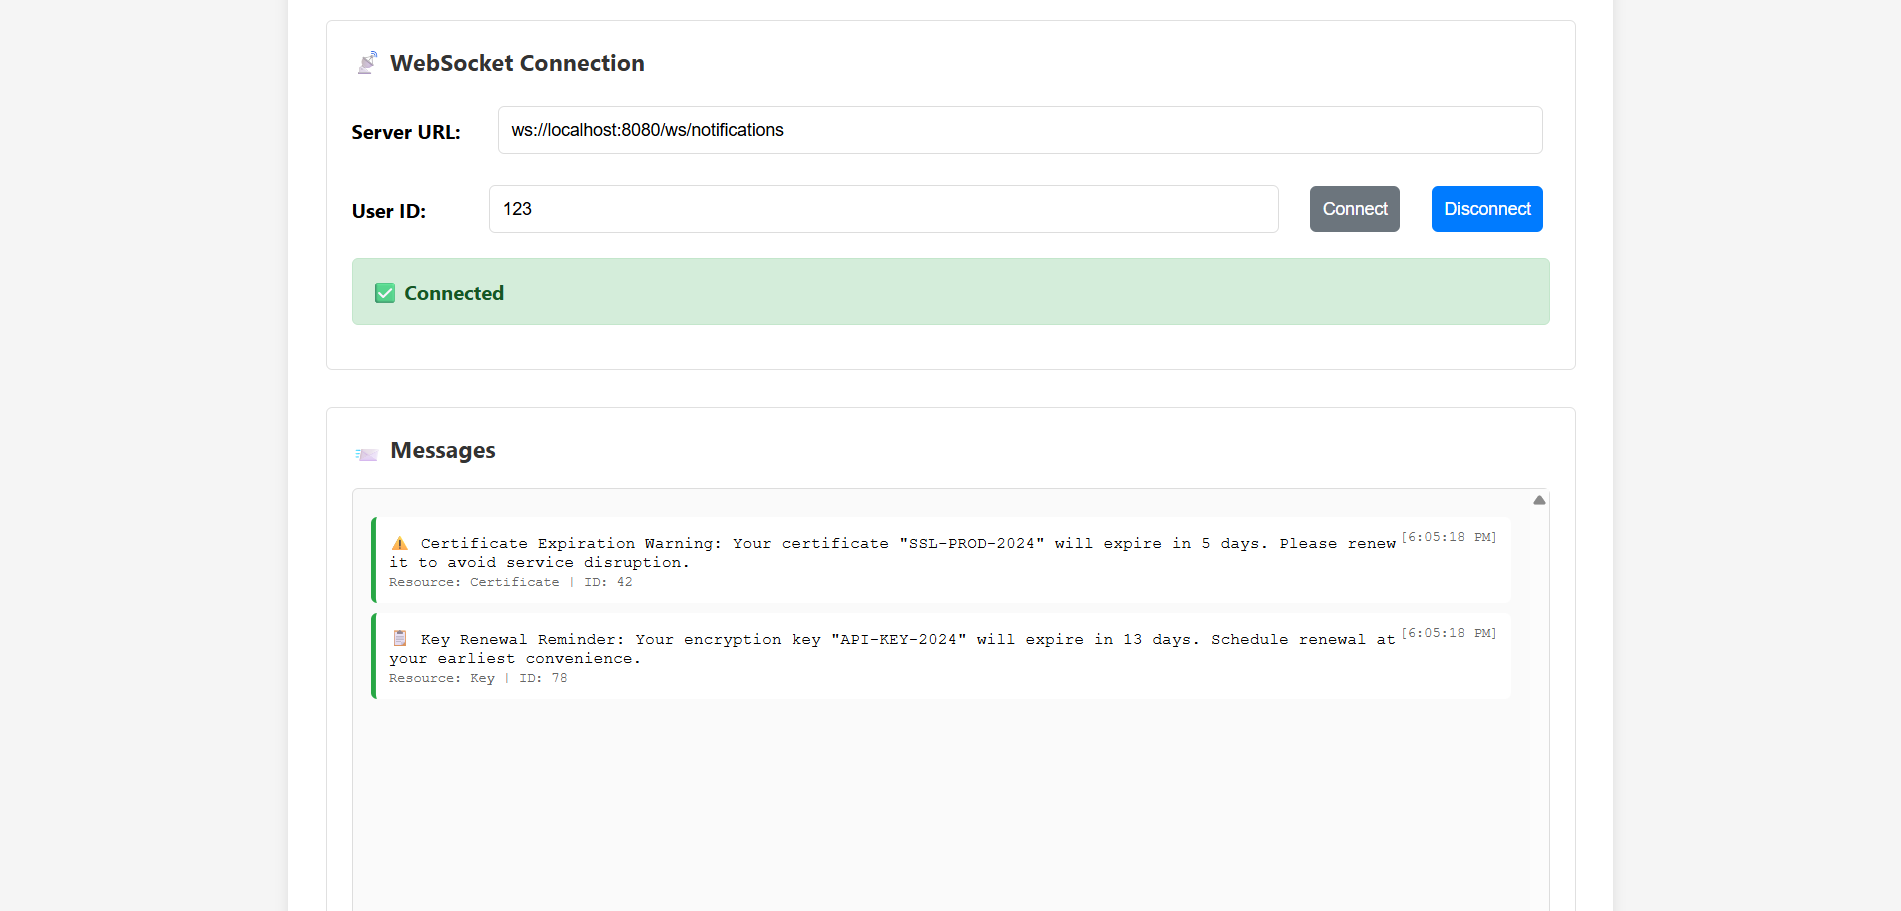
\includegraphics[width=1\textwidth]{images/websocket_message.png}
    \caption{WebSocket Real-time Notification Delivery}
    \label{fig:websocket_message}
\end{figure}

The message delivery test demonstrates successful real-time notification transmission through the WebSocket connection. The structured message format includes notification details, resource information, and timing data, providing users with comprehensive information about expiring cryptographic resources.

\section{Manual Job Execution Endpoints}

For testing and administrative purposes, the system provides endpoints to manually trigger the background jobs that normally run on scheduled intervals.

\subsection{Process Notifications Endpoint}

\textbf{POST /v1/notifications/jobs/process-notifications}

This endpoint manually triggers the notification processing job, which evaluates pending notifications and sends those matching the current day in the Fibonacci sequence.

\subsection{Resource Discovery Endpoint}

\textbf{POST /v1/notifications/jobs/discover-all-resources}

This endpoint manually triggers the resource discovery job, which scans the database for expiring certificates and keys and creates appropriate notification records.

These administrative endpoints proved essential during development and testing phases, allowing for controlled execution of the automated processes.

\section*{Conclusion}

This chapter presented the practical implementation of the notification system, focusing on the development of REST API endpoints and WebSocket functionality. The implementation successfully provides the necessary interfaces for immediate and scheduled notification management, resource status updates, and real-time communication.

The use of modern development tools and frameworks facilitated efficient implementation while maintaining code quality and system reliability. The comprehensive API testing with Bruno validated endpoint functionality and request/response handling, ensuring that the system meets the specified requirements.

The WebSocket implementation adds real-time capability to the notification system, enhancing user experience by providing immediate awareness of critical resource expirations. The combination of REST APIs and WebSocket communication creates a comprehensive notification platform that addresses both immediate and long-term cryptographic resource management needs.

The implemented endpoints integrate seamlessly with the existing KMS architecture while providing the foundation for automated notification processes described in the previous chapters. This implementation represents a significant step toward proactive cryptographic resource lifecycle management within the Renault Group's security infrastructure.